



\subsection{Numerics}

From a numerical point of view, it is convenient to solve for the
eigenmodes of the linear operator $\hat q$ and $\hat a_\pm = \hat a
/2 \pm \omega_l \hat d /(2i)$.
%
We thus consider the following modified governing equations
\begin{eqnarray}
\bigl( \p_t  + \fdiss(\kk) \bigl) \hat q  
&=& \hat N_q  ,\label{eqqnum} \\
\bigl( \p_t  + \fdiss(\kk) \pm  i \omega_l \bigl)  \hat a_\pm  
&=& \hat N_{\pm} + \hat f_{\pm}, \label{eqapmnum}
\end{eqnarray}
where $\hat f_{\pm}$ are forcing terms and %
$\hat N_q$ and %
$\hat N_\pm = \hat N_a /2 \pm \omega_l \hat N_d/(2i)$ %
are non-linear terms computed from %
$\hat \NN_\uu = - \zeta \eez \wedge \uu - \bnabla |\uu|^2/2$ and %
$\hat N_\eta = - \bnabla \cdot (\eta \uu)$.
%
We have removed the Newtonian viscous operator in (\ref{eq_uu}) and
added more general dissipative operators in (\ref{eq_uu}) and
(\ref{eq_h}).  There is no strong physical motivations for this
modification but, as discussed by \cite{FargeSadourny1989}, molecular
dissipation of the form $\nu \bnabla^2 \uu$ is not necessarily a
relevant model of the actual small-scale dissipation for shallow-water
flows, which should rather be described as a transition from
two-dimensional to three-dimensional motions before reaching the
scales where dissipation actually occurs.




Equations (\ref{eqqnum}-\ref{eqapmnum}) are simulated by means of a
pseudo-spectral method with periodic boundary conditions.
%
Time advancement is carried out by a classical fourth-order
Runge-Kutta scheme for the nonlinear term and an exact integration for
the linear and dissipative terms.  This explicit integration is
especially interesting at very high resolution and very large $c$ when
the shortest waves are very fast with frequency of the order of
$\omega \simeq c \max(k)$.
%
We use an adaptable time step method which maximizes the time step
over a standard Courant-Friedrichs-Lewy condition
\cite[]{Lundbladh1999, AugierChomazBillant2012}.
%
Most of the aliasing is removed by truncating 8/9 of the modes along
each direction \cite[for a detail discussion on the issues of the
non-conservation of the non-quadratic energy and the aliasing errors
in the truncated one-layer shallow water model,
see][]{FargeSadourny1989}.




\subsection{Forced dissipative statistically stationary simulations}

We have carried out a number of simulations 
with large-scale forcing and small-scale dissipation
for different resolutions and different values of the wave speed.
%
The resolution is characterized by the number of nodes in the each
direction, $n$, and has been varied from 240 to 7680.
%
The wave speed $c$ has been varied over two orders of magnitude from
10 to 1000.
%
Table~\ref{tab} presents the parameters for a set of representative
simulations.

\begin{table}
  \begin{center}
% \def~{\hphantom{0}}
\begin{tabular}{cc@{\hskip 8mm}c@{\hskip 8mm}cccc@{\hskip 8mm}cc}
$n$ & $c$ & $\nu_8$ & $\eps$ & $\displaystyle\frac{\kmax}{\kdiss}$ & $\displaystyle\frac{\kdiss}{k_f}$ & $F_f$ & $\min h$ & $\displaystyle\frac{\max |\uu|}{c}$ \\[3mm]
~960 &   10 & 1.5e-10 & 1.03 & 2.46 &  29 &  0.111 & 0.25 & 0.96 \\
1920 &   10 & 9.6e-13 & 1.00 & 2.46 &  58 &  0.110 & 0.37 & 0.92 \\
3840 &   10 & 6.0e-15 & 1.01 & 2.46 & 116 &  0.110 & 0.39 & 1.01 \\
7680 &   10 & 3.7e-17 & 1.03 & 2.46 & 231 &  0.111 & 0.32 & 0.95 \\[1mm]
~960 &   20 & 1.5e-10 & 0.98 & 2.47 &  29 &  0.055 & 0.65 & 0.51 \\
1920 &   20 & 9.6e-13 & 0.84 & 2.48 &  57 &  0.052 & 0.66 & 0.81 \\
3840 &   20 & 6.0e-15 & 0.99 & 2.46 & 115 &  0.055 & 0.56 & 0.68 \\[1mm]
~960 &   40 & 1.5e-10 & 0.99 & 2.46 &  29 &  0.027 & 0.81 & 0.24 \\
1920 &   40 & 9.6e-13 & 1.01 & 2.46 &  58 &  0.028 & 0.78 & 0.28 \\
3840 &   40 & 6.0e-15 & 0.98 & 2.47 & 115 &  0.027 & 0.77 & 0.29 \\
7680 &   40 & 3.7e-17 & 0.94 & 2.47 & 230 &  0.027 & 0.76 & 0.32 \\[1mm]
~960 &  100 & 1.5e-10 & 0.99 & 2.46 &  29 &  0.011 & 0.89 & 0.09 \\
1920 &  100 & 9.6e-13 & 0.98 & 2.47 &  58 &  0.011 & 0.90 & 0.11 \\
3840 &  100 & 6.0e-15 & 0.97 & 2.47 & 115 &  0.011 & 0.87 & 0.13 \\[1mm]
~960 &  200 & 1.5e-10 & 0.99 & 2.46 &  29 &  0.005 & 0.95 & 0.05 \\
1920 &  200 & 9.6e-13 & 0.99 & 2.46 &  58 &  0.005 & 0.94 & 0.06 \\
3840 &  200 & 6.0e-15 & 0.90 & 2.47 & 115 &  0.005 & 0.94 & 0.06 \\[1mm]
~960 &  400 & 1.5e-10 & 0.97 & 2.47 &  29 &  0.003 & 0.97 & 0.03 \\
1920 &  400 & 9.6e-13 & 0.99 & 2.46 &  58 &  0.003 & 0.96 & 0.03 \\[1mm]
~960 & 1000 & 1.5e-10 & 1.16 & 2.45 &  29 &  0.001 & 0.98 & 0.01 \\
1920 & 1000 & 9.6e-13 & 0.91 & 2.47 &  57 &  0.001 & 0.98 & 0.01 \\
\end{tabular}
\caption{Overview of parameters for a set of representative simulations. 
The number of nodes in the each direction is denoted by $n$. 
The size of the numerical domain is equal to $L_h = 50$.
Only the wave numbers $5\delta k\leqslant|\kk|\leqslant8\delta k$ are forced
and the forcing wave number is defined as 
$k_f \equiv 6 \delta k$ 
corresponding to a characteristic forcing scale of approximately 
$L_f \equiv \pi/k_f = 3.57$.
%
$F_f = \eps^{1/3}/({k_f}^{1/3}c)$ is the forcing Froude number and
$\max |\uu|/c$ is the spatial and temporal maximum of a local Froude
number.  }
\label{tab}
\end{center}
\end{table}



The ageostrophic variable $a$ is forced in a shell in spectral space
corresponding to relatively small wave numbers $5\delta k\leqslant
|\kk| \leqslant 8\delta k$, where $\delta k = 2\pi/L_h$.
%
\Add{In the following, we use $L_h = 50$ in order to obtain a
characteristic forcing wave number of order unity, $k_f \equiv 6
\delta k \simeq 0.75$. The corresponding forcing scale is $L_f \equiv
\pi/k_f \simeq 4.2$.}
%
Since only the ageostrophic variable is forced ($\hat f_d = 0$),%
(i) only the thickness fluctuation $\eta$ is forced in the
non-rotating case and %
(ii) the force terms in (\ref{eqapmnum}) are simply equal to $\hat
f_\pm = \hat f_a/2$.
%
In order to compute the force $\hat f_a$, we start from a
pre-normalized force $\hat f_{0}$ obtained from a normal random
process decorrelated in time.
%
The force is then normalized such that the quadratic part of the total
energy $\langle|\uu|^2 + c^2 \eta^2\rangle/2$ is injected at a
constant rate.
%
The spectral injection rate of the quadratic energy averaged over one
time step is (see appendix~\ref{app_comp})
\begin{equation}
P_q(\kk, t) 
= 
\Re\{ \hat \uu(\kk)^* \cdot \hat \ff(\kk) 
+
c^2 \hat \eta(\kk)^* \hat f_\eta(\kk) \}
+ 
(|\hat\ff|^2 + c^2 |\hat f_\eta|^2) \delta t /2,
\end{equation}
where $\Re$ denotes the real part.
%
Writing $\hat f_a = \alpha \hat f_{0}$, it is straightforward to solve
a second-order equation for the coefficient $\alpha$ in order to fix
the injection rate $\Add{P_0 \equiv} \sum_\kk P_q(\kk, t)$ to unity.


The energy is dissipated at the smallest resolved scales by a
hyper-viscous operator, corresponding to a dissipative frequency equal
to $\fdiss(\kk) = \nu_n |\kk|^n$, with $n = 8$.  The value of the
hyperviscosity $\nu_8$ is chosen such as the hyper-Kolmogorov wave
number
\begin{equation}
k_{Kn} = \left( \frac{{\nu_n}^3}{\eps} \right)^\frac{1}{3n-2},
\end{equation}
is well resolved, $\kdiss =k_{K8} \simeq \kmax/ 2.5$, where $\kmax =
(8/9)\pi n/L_h$ is the maximum resolved wave number.

We have observed that when only the waves are forced, the vorticity
does not increase and that when the vorticity is small enough, it does
not significantly influence the waves.  Therefore, we have chosen not
to simulate a negligible vorticity field and to only solve equations
(\ref{eqapmnum}) with $\zeta = 0$.







\begin{figure}
\centerline{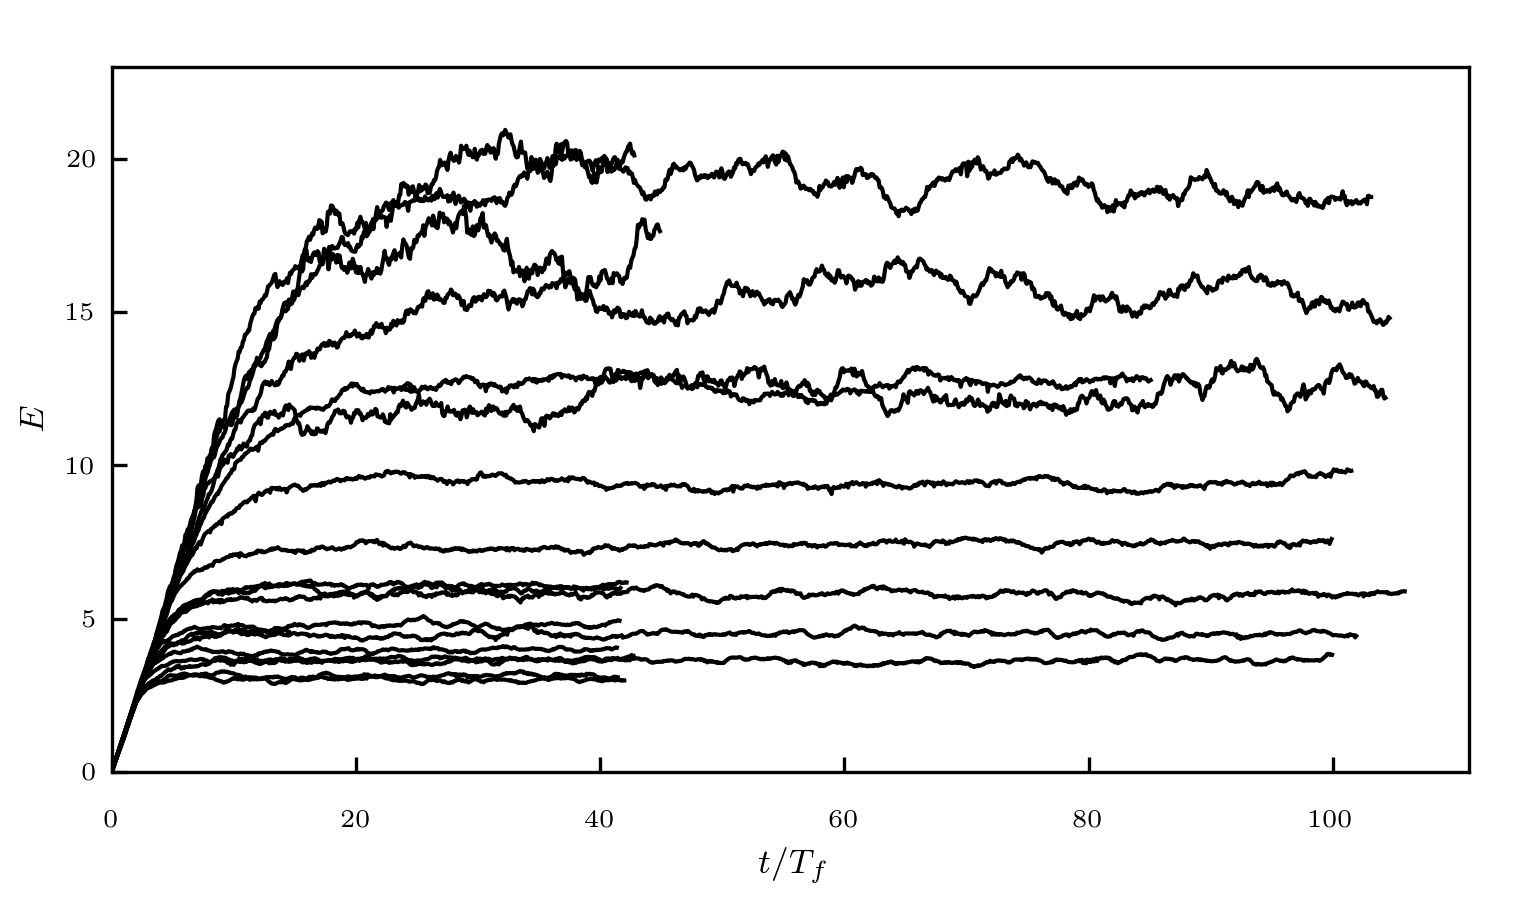
\includegraphics[width=13cm]{../Figs/fig_Emean_time}}
\caption{Space averaged energy 
$\langle h|\uu|^2 + c^2 h^2 \rangle/2$ versus time 
for different wave speeds $c$ and resolutions $n$.
%
The energy and the time are normalized by 
$E_f\equiv (P_0/k_f)^{2/3}$ and $T_f\equiv (P_0 {k_f}^2)^{-1/3}$,
with $P_0 = 1 \simeq \eps$.
%
The colors corresponds to different wave speeds as indicated in the figure
$c= 10$, 20, 40, 70, 100, 200, 400, 700 and 1000.
%
The different resolutions are represented by different types of lines:
\Add{thin continuous lines, $n = 240$;
thick dashed lines, $n = 480$;
thin dotted lines, $n = 960$;
thick continuous lines, $n = 1920$;
thin dashed lines, $n = 3840$;
thick dotted lines, $n = 5760$ 
and
thin dotted dashed lines, $n = 7680$.}
}
\label{fig_Evstime}
\end{figure}






The time evolution of the instantaneous total energy is shown in
figure~\ref{fig_Evstime} for different wave speeds $c$.
%
The resolution \Add{and the dissipation wave number are} progressively
increased: %
$n = 240$ ($0\leqslant t/T_f \leqslant 100$), %
$n = 480$ ($100\leqslant t/T_f \leqslant 125$), %
$n = 960$ ($125\leqslant t/T_f \leqslant 140$), %
$n = 1920$, %
$n = 3840$, %
$n = 5760$ and %
$n = 7680$\Add{, where $T_f\equiv
(P_0 {k_f}^2)^{-1/3}$ is the characteristic forcing time}.
%
Each time the resolution is increased, the energy first sharply
increases and then fluctuates.  For most of the simulations, it is
clear that a statistically stationary regime is reached.
%
However, 
%
\Remove{in the relatively short simulations at the highest
resolution for the largest wave speeds ($n = 1920$, $c = 700$ and
1000),}
%
\Add{for some relatively short simulations with very large wave speed
and/or very large resolution,}
%
there are large fluctuations and it is not absolutely certain whether
a statistically stationary regime is reached.
%
\Add{This is in particular the case for the simulations for $c = 700$, $n
= 1920$ (thick red continuous line), $c = 200$, $n = 3840$ (thin
magenta dashed line) and $c=40$, $n = 7680$ (thin blue dotted dashed
line).}
%
\Add{Note that these simulations are already quite numerically
costly. For example, the simulation for $c=1000$ and $n = 1920$
during slightly less than $20T_f$ corresponds to approximately
$8\times 10^5$ time steps.}


Since the energy is injected at large scales and dissipated only at
the smallest resolved scales, the existence of a statistically
stationary regime implies a downscale flux of energy, which is equal
to the large-scale energy injection rate.
%
For the same energy injection rate and resolution, the mean energy
increases with the wave speed, implying that when $c$ increases the
mean energy has to be larger to lead to the same downscale energy
flux.
%
The results presented in the following are from the statistically
stationary regime.  Apart from the snapshots, all shown quantities are
averaged over a period corresponding to this regime.



Table~\ref{tab} presents numerical and physical quantities for a set
of representative simulations.
%
We characterize the simulations by the forcing Froude number
\begin{equation}
F_f \Add{\equiv} \frac{\eps^{1/3}}{{k_f}^{1/3}c}.
\end{equation}
\Add{Since the characteristic forcing wave number and the dissipation
rate are approximately equal to $k_f \equiv 6 \delta k \simeq 0.75$
and $\eps \simeq P_0 = 1$, the forcing Froude number is approximately
inversely proportional to the wave speed: $F_f \simeq 1.1/c$. This
allows us to simply use the wave speed to denote the simulations.}
% where $k_f \equiv 6 \delta k = 0.75$ is a wave number characterizing
% the forcing.
%
The ratio $\kdiss/k_f$ gives an order of magnitude of the width of the
inertial range.  It is a physical quantity related to the numerical
resolution on which the flow can depend.
%
Table~\ref{tab} also displays the minimum thickness $\min(h)$
characterizing the importance of the non-quadraticity of the energy,
and $\max(|\uu|/c)$, which can be interpreted as the maximum of a
local Froude number.




